\documentclass[11pt]{article}\usepackage[]{graphicx}\usepackage[]{color}
%% maxwidth is the original width if it is less than linewidth
%% otherwise use linewidth (to make sure the graphics do not exceed the margin)
\makeatletter
\def\maxwidth{ %
  \ifdim\Gin@nat@width>\linewidth
    \linewidth
  \else
    \Gin@nat@width
  \fi
}
\makeatother

\definecolor{fgcolor}{rgb}{0.345, 0.345, 0.345}
\newcommand{\hlnum}[1]{\textcolor[rgb]{0.686,0.059,0.569}{#1}}%
\newcommand{\hlstr}[1]{\textcolor[rgb]{0.192,0.494,0.8}{#1}}%
\newcommand{\hlcom}[1]{\textcolor[rgb]{0.678,0.584,0.686}{\textit{#1}}}%
\newcommand{\hlopt}[1]{\textcolor[rgb]{0,0,0}{#1}}%
\newcommand{\hlstd}[1]{\textcolor[rgb]{0.345,0.345,0.345}{#1}}%
\newcommand{\hlkwa}[1]{\textcolor[rgb]{0.161,0.373,0.58}{\textbf{#1}}}%
\newcommand{\hlkwb}[1]{\textcolor[rgb]{0.69,0.353,0.396}{#1}}%
\newcommand{\hlkwc}[1]{\textcolor[rgb]{0.333,0.667,0.333}{#1}}%
\newcommand{\hlkwd}[1]{\textcolor[rgb]{0.737,0.353,0.396}{\textbf{#1}}}%
\let\hlipl\hlkwb

\usepackage{framed}
\makeatletter
\newenvironment{kframe}{%
 \def\at@end@of@kframe{}%
 \ifinner\ifhmode%
  \def\at@end@of@kframe{\end{minipage}}%
  \begin{minipage}{\columnwidth}%
 \fi\fi%
 \def\FrameCommand##1{\hskip\@totalleftmargin \hskip-\fboxsep
 \colorbox{shadecolor}{##1}\hskip-\fboxsep
     % There is no \\@totalrightmargin, so:
     \hskip-\linewidth \hskip-\@totalleftmargin \hskip\columnwidth}%
 \MakeFramed {\advance\hsize-\width
   \@totalleftmargin\z@ \linewidth\hsize
   \@setminipage}}%
 {\par\unskip\endMakeFramed%
 \at@end@of@kframe}
\makeatother

\definecolor{shadecolor}{rgb}{.97, .97, .97}
\definecolor{messagecolor}{rgb}{0, 0, 0}
\definecolor{warningcolor}{rgb}{1, 0, 1}
\definecolor{errorcolor}{rgb}{1, 0, 0}
\newenvironment{knitrout}{}{} % an empty environment to be redefined in TeX

\usepackage{alltt}
\usepackage{amsmath}
\usepackage{amssymb}
\usepackage{geometry}
\usepackage{graphicx}
\usepackage{bm}
\usepackage{url}
\usepackage{enumerate}
\usepackage{hyperref}
\IfFileExists{upquote.sty}{\usepackage{upquote}}{}
\begin{document}

\setlength\parindent{0pt}

\large \textbf{Lab 2: Simulating SLR}\\
\normalsize STAT 632, Spring 2020\\

In this lab we consider simulating data from the the following simple linear regression (SLR) model:
$$Y = \beta_0 + \beta_1 x + e = 2 + 3x + e, \text{ where } e \sim N(0, 25),$$
that is $Var(e) = \sigma^2 = 25$.  This is the equation for the population regression line, which, in practice, is unknown.  For the simulation, we can generate data from this model, and then obtain estimates of the parameters using the least squares method.  This will enable us to investigate and gain insight into properties of the SLR model.  

%Recall that there is some hypothetic population regression line given $Y = \beta_0 + \beta_1 x + e$, where $e \sim N(0,\sigma^2)$.  In practice, we guess that the data are generate by this model, and we use the data to estimate the parameters.  With simulation, we can specifiy the population regression line and generate data from that model.  Simulations provide a way to investigate poperties of our model. 

\begin{knitrout}
\definecolor{shadecolor}{rgb}{0.969, 0.969, 0.969}\color{fgcolor}\begin{kframe}
\begin{alltt}
\hlstd{n} \hlkwb{<-} \hlnum{50} \hlcom{# sample size}
\hlstd{beta0} \hlkwb{<-} \hlnum{2} \hlcom{# population intercept}
\hlstd{beta1} \hlkwb{<-} \hlnum{3} \hlcom{# population slope}
\hlstd{sigma} \hlkwb{<-} \hlnum{5}

\hlkwd{set.seed}\hlstd{(}\hlnum{99}\hlstd{)}
\hlstd{x} \hlkwb{<-} \hlkwd{rnorm}\hlstd{(n)}
\hlstd{e} \hlkwb{<-} \hlkwd{rnorm}\hlstd{(n,} \hlkwc{mean}\hlstd{=}\hlnum{0}\hlstd{,} \hlkwc{sd}\hlstd{=sigma)}
\hlstd{y} \hlkwb{<-} \hlstd{beta0} \hlopt{+} \hlstd{beta1} \hlopt{*} \hlstd{x} \hlopt{+} \hlstd{e}

\hlcom{# estimate SLR model from simulated data}
\hlstd{lm1} \hlkwb{<-} \hlkwd{lm}\hlstd{(y} \hlopt{~} \hlstd{x)}
\hlkwd{summary}\hlstd{(lm1)}
\end{alltt}
\begin{verbatim}
## 
## Call:
## lm(formula = y ~ x)
## 
## Residuals:
##    Min     1Q Median     3Q    Max 
## -8.296 -2.693  0.224  1.991  9.112 
## 
## Coefficients:
##             Estimate Std. Error t value Pr(>|t|)    
## (Intercept)   2.3255     0.5447   4.269 9.21e-05 ***
## x             3.4105     0.5234   6.515 4.07e-08 ***
## ---
## Signif. codes:  0 '***' 0.001 '**' 0.01 '*' 0.05 '.' 0.1 ' ' 1
## 
## Residual standard error: 3.737 on 48 degrees of freedom
## Multiple R-squared:  0.4693,	Adjusted R-squared:  0.4583 
## F-statistic: 42.45 on 1 and 48 DF,  p-value: 4.072e-08
\end{verbatim}
\end{kframe}
\end{knitrout}

The scatterplot below shows the population regression line (solid) and the least squares estimate (dashed).

\begin{knitrout}
\definecolor{shadecolor}{rgb}{0.969, 0.969, 0.969}\color{fgcolor}\begin{kframe}
\begin{alltt}
\hlkwd{par}\hlstd{(}\hlkwc{mar}\hlstd{=}\hlkwd{c}\hlstd{(}\hlnum{4.5}\hlstd{,}\hlnum{4.5}\hlstd{,}\hlnum{2}\hlstd{,}\hlnum{2}\hlstd{))} \hlcom{#adjust margins}
\hlkwd{plot}\hlstd{(y} \hlopt{~} \hlstd{x)}
\hlkwd{abline}\hlstd{(beta0, beta1,} \hlkwc{lwd}\hlstd{=}\hlnum{1.5}\hlstd{,} \hlkwc{lty}\hlstd{=}\hlnum{1}\hlstd{)} \hlcom{# population regression line}
\hlkwd{abline}\hlstd{(lm1,} \hlkwc{lwd}\hlstd{=}\hlnum{1.5}\hlstd{,} \hlkwc{lty}\hlstd{=}\hlnum{2}\hlstd{)} \hlcom{# least squares estimate}
\hlkwd{legend}\hlstd{(}\hlstr{'bottomright'}\hlstd{,} \hlkwc{lwd}\hlstd{=}\hlnum{1.5}\hlstd{,} \hlkwc{lty}\hlstd{=}\hlkwd{c}\hlstd{(}\hlnum{1}\hlstd{,} \hlnum{2}\hlstd{),} \hlkwd{c}\hlstd{(}\hlstr{'Population'}\hlstd{,} \hlstr{'Estimate'}\hlstd{))}
\end{alltt}
\end{kframe}
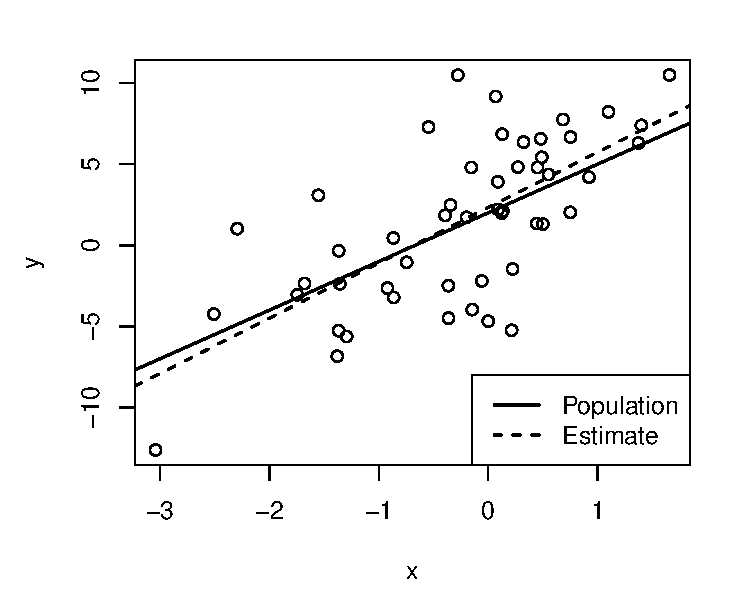
\includegraphics[width=\maxwidth]{figure/unnamed-chunk-3-1} 

\end{knitrout}

\textbf{Your turn:}  Generate another simulated data set of size $n=50$ from the SLR model $Y = 2 + 3x + e$, where $e \sim N(0, 25)$.  Make a scatterplot with your simulated data, and add the least squares line and population regression line.\\    
\clearpage

We can repeatedly simulate data from the SLR model, $Y = 2 + 3x + e$.  Each simulated data set will give a slightly different least squares estimate of the slope and intercept of the line.  The \texttt{for loop} below generates 10,000 simulated data sets from the SLR model.  The least squares regression line is estimated from each data set.  This gives 10,000 estimates of the population regression line; that is, 10,000 least squares estimates of the slope and intercept.  Note that the values of the explanatory variable $x$ are considered fixed in SLR, so the $x$ values are only specified once (before running the loop).


\begin{knitrout}
\definecolor{shadecolor}{rgb}{0.969, 0.969, 0.969}\color{fgcolor}\begin{kframe}
\begin{alltt}
\hlkwd{set.seed}\hlstd{(}\hlnum{99}\hlstd{)}
\hlstd{beta1hat} \hlkwb{<-} \hlkwd{rep}\hlstd{(}\hlnum{0}\hlstd{,} \hlnum{10000}\hlstd{)} \hlcom{# initialize vector of slope estimates}
\hlstd{x} \hlkwb{<-} \hlkwd{rnorm}\hlstd{(n)} \hlcom{# simulate x values}
\hlkwa{for}\hlstd{(i} \hlkwa{in} \hlnum{1}\hlopt{:}\hlnum{10000}\hlstd{) \{}
  \hlstd{e} \hlkwb{<-} \hlkwd{rnorm}\hlstd{(n,} \hlkwc{mean}\hlstd{=}\hlnum{0}\hlstd{,} \hlkwc{sd}\hlstd{=sigma)}
  \hlstd{y} \hlkwb{<-} \hlstd{beta0} \hlopt{+} \hlstd{beta1} \hlopt{*} \hlstd{x} \hlopt{+} \hlstd{e}
  \hlstd{lm_i} \hlkwb{<-} \hlkwd{lm}\hlstd{(y} \hlopt{~} \hlstd{x)}
  \hlstd{beta1hat[i]} \hlkwb{<-} \hlkwd{as.numeric}\hlstd{(}\hlkwd{coef}\hlstd{(lm_i)[}\hlnum{2}\hlstd{])}
\hlstd{\}}
\end{alltt}
\end{kframe}
\end{knitrout}

Below is a histogram of the 10,000 least squares estimates of the slope (i.e., the simulated sampling distribution).  Note that the estimates of the slope are centered around the population slope, $\beta_1 = 3$, and normally distributed.  

\begin{knitrout}
\definecolor{shadecolor}{rgb}{0.969, 0.969, 0.969}\color{fgcolor}\begin{kframe}
\begin{alltt}
\hlkwd{par}\hlstd{(}\hlkwc{mar}\hlstd{=}\hlkwd{c}\hlstd{(}\hlnum{4}\hlstd{,}\hlnum{4}\hlstd{,}\hlnum{1}\hlstd{,}\hlnum{1}\hlstd{))} \hlcom{#adjust margins}
\hlkwd{hist}\hlstd{(beta1hat,} \hlkwc{main}\hlstd{=}\hlstr{''}\hlstd{)}
\hlkwd{abline}\hlstd{(}\hlkwc{v}\hlstd{=}\hlnum{3}\hlstd{,} \hlkwc{col}\hlstd{=}\hlstr{'blue'}\hlstd{,} \hlkwc{lwd}\hlstd{=}\hlnum{2}\hlstd{)}
\end{alltt}
\end{kframe}
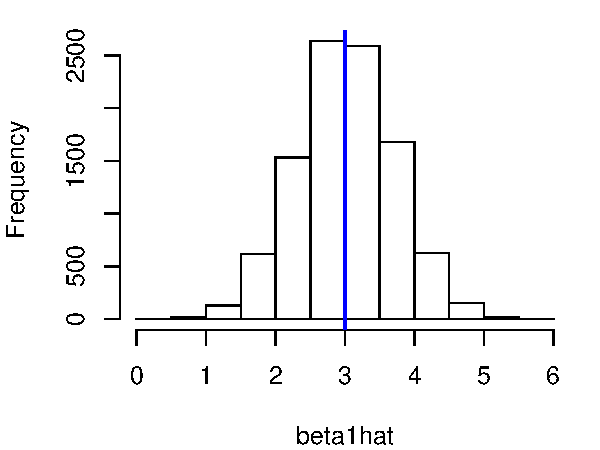
\includegraphics[width=\maxwidth]{figure/unnamed-chunk-5-1} 

\end{knitrout}


\clearpage
The variance of the 10,000 estimates of the slope is also approximately equal to true variance given by the formula $Var(\hat{\beta}_1) = \sigma^2 / SXX$ where $SXX = \sum_{i=1}^n (x_i - \bar{x})^2$.
\begin{knitrout}
\definecolor{shadecolor}{rgb}{0.969, 0.969, 0.969}\color{fgcolor}\begin{kframe}
\begin{alltt}
\hlcom{# variance of the slope estimates}
\hlkwd{var}\hlstd{(beta1hat)}
\end{alltt}
\begin{verbatim}
## [1] 0.487108
\end{verbatim}
\begin{alltt}
\hlcom{# true (analytic) variance}
\hlstd{SXX} \hlkwb{<-} \hlkwd{sum}\hlstd{((x} \hlopt{-} \hlkwd{mean}\hlstd{(x))}\hlopt{^}\hlnum{2}\hlstd{)}
\hlstd{sigma}\hlopt{^}\hlnum{2} \hlopt{/} \hlstd{SXX}
\end{alltt}
\begin{verbatim}
## [1] 0.4905309
\end{verbatim}
\end{kframe}
\end{knitrout}





\end{document}
